\documentclass[oneside, 11pt]{article}

\usepackage[T1]{fontenc}
\usepackage[utf8]{inputenc}
\usepackage[dutch]{babel}

\usepackage{fouriernc}
\usepackage[detect-all, load-configurations=binary,
            separate-uncertainty=true, per-mode=symbol,
            retain-explicit-plus, range-phrase={ tot }]{siunitx}

\usepackage{setspace}
\setstretch{1.2}

\setlength{\parskip}{\smallskipamount}
\setlength{\parindent}{0pt}

\usepackage{geometry}
\geometry{marginparwidth=0.5cm, verbose, a4paper, tmargin=3cm, bmargin=3cm, lmargin=2cm, rmargin=2cm}

\usepackage{float}

\usepackage[fleqn]{amsmath}
\numberwithin{equation}{section}
\numberwithin{figure}{section}

\usepackage{graphicx}
\graphicspath{{Figures/}}
\usepackage{subfig}

\usepackage{tikz}
\usetikzlibrary{plotmarks}

\usepackage{fancyhdr}
\pagestyle{fancy}
\fancyhf{}
\rhead{\thepage}
\renewcommand{\footrulewidth}{0pt}
\renewcommand{\headrulewidth}{0pt}

\usepackage{relsize}
\usepackage{xspace}
\usepackage{url}

\newcommand{\figref}[1]{Figuur~\ref{#1}}

\newcommand{\hisparc}{\textsmaller{HiSPARC}\xspace}
\newcommand{\kascade}{\textsmaller{KASCADE}\xspace}
\newcommand{\sapphire}{\textsmaller{SAPPHiRE}\xspace}
\newcommand{\jsparc}{\textsmaller{jSparc}\xspace}
\newcommand{\hdf}{\textsmaller{HDF5}\xspace}
\newcommand{\aires}{\textsmaller{AIRES}\xspace}
\newcommand{\csv}{\textsmaller{CSV}\xspace}
\newcommand{\python}{\textsmaller{PYTHON}\xspace}
\newcommand{\corsika}{\textsmaller{CORSIKA}\xspace}
\newcommand{\labview}{\textsmaller{LabVIEW}\xspace}
\newcommand{\daq}{\textsmaller{DAQ}\xspace}
\newcommand{\adc}{\textsmaller{ADC}\xspace}
\newcommand{\adcs}{\textsmaller{ADC}s\xspace}
\newcommand{\Adcs}{A\textsmaller{DC}s\xspace}
\newcommand{\hi}{\textsc{h i}\xspace}
\newcommand{\hii}{\textsc{h ii}\xspace}
\newcommand{\mip}{\textsmaller{MIP}\xspace}
\newcommand{\hisparcii}{\textsmaller{HiSPARC II}\xspace}
\newcommand{\hisparciii}{\textsmaller{HiSPARC III}\xspace}
\newcommand{\pmt}{\textsmaller{PMT}\xspace}
\newcommand{\pmts}{\textsmaller{PMT}s\xspace}

\DeclareSIUnit{\electronvolt}{\ensuremath{\mathrm{e\!\!\:V}}}

\DeclareSIUnit{\unitsigma}{\ensuremath{\sigma}}
\DeclareSIUnit{\mip}{\textsmaller{MIP}}
\DeclareSIUnit{\adc}{\textsmaller{ADC}}

\DeclareSIUnit{\gauss}{G}
\DeclareSIUnit{\parsec}{pc}
\DeclareSIUnit{\year}{yr}



\title{Stationsplattegrond}
\author{A.P.L.S. de Laat, N.G. Schultheiss}
\docwerkblad{3}{SP}
\version{2.1}

\begin{document}

\maketitle

\section{Inleiding}

Een \hisparc station bestaat uit twee of vier detectoren die op het dak van een
(school)gebouw staan. Elk paar detectoren is aangesloten op \hisparc II of
\hisparc III electronica. De \hisparc electronica is in twee varianten
beschikbaar, namelijk als master en als slave. Een \hisparc station heeft
altijd een \hisparc master, hierop wordt de \gps antenne aangesloten. De
electronica kan twee detectoren uitlezen, een station met vier detectoren heeft
daarom ook een slave nodig. De master en slave werken samen als een eenheid. De
master en eventuele slave van een station zijn aangesloten op een meetcomputer,
die de metingen naar de \hisparc server stuurt. Met de computer zijn de
aangesloten units ook af te regelen.

Met de \gps antenne is de locatie van een station te bepalen.
\gps satellieten zenden radiosignalen uit, in dit signaal wordt de tijd
van de satelliet op het moment van uitzenden op 1 ns nauwkeurig meegestuurd.
Met het verschil tussen de aankomsttijd van het signaal en de lokale
tijd van de antenne zijn de afstanden uit te rekenen. Deze tijd kunnen we
ook gebruiken om  vast te leggen wanneer de detectoren iets meten.

Omdat de \gps antenne zowel de plaats als de tijd van een station definieert,
wordt de plaats van de detectoren ten opzichte van de \gps antenne vastgelegd.
De posities van de detectoren worden niet automatisch bepaald zoals die van de
\gps. De posities van de detectoren moeten met de hand gemeten worden. De
posities van de detectoren zijn nodig voor de data analyse.


\section{Kaarten}

De plaats van de \gps antenne wordt via het internet naar de \hisparc
server gestuurd. De configuratie van het station is in een Firefox,
Chrome of Safari browser op te halen op:

\texttt{\small{http://data.hisparc.nl/api/station/}}{\small{\{Stationsnummer\}}}

Op de plaats van \{Stationsnummer\} vul je het stationsnummer in. Let
op: Internet Explorer werkt niet!

Met enig zoeken zijn de Oosterlengte (longitude) en Noorderbreedte
(latitude), beide in graden te vinden. De hoogte (altitude) wordt in
meter vanaf de WGS 84 ellipsoïde gemeten. Deze ellipsoïde ligt in
Amsterdam tientallen meters onder NAP (het Nieuw Amsterdams Peil).

\begin{minipage}[t]{1\columnwidth}%

\paragraph{Opdracht 1:}

Bepaal hoever de \gps antenne van het te meten station boven de WGS 84
ellipsoïde ligt en hoever dit boven NAP is.

\begin{center}
    \rule{\textwidth}{0.3mm}\\
    \rule{\textwidth}{0.3mm}\\
    \rule{\textwidth}{0.3mm}\\
\end{center}

\end{minipage}


\section{Het meten van de opstelling}


\subsection{Benodigdheden}

Om de opstelling te meten hebben we het volgende nodig:

\begin{itemize}
    \item Kompas
    \item Meetlint (liefst langer dan \SI{10}{\meter})
    \item Veiligheidsmateriaal (harnas + zekeringslijn)
    \item Pen en papier om de metingen te noteren
    \item Sleutels van de `skiboxen'
\end{itemize}

\subsection{Veiligheid}

De verrichtingen op het dak moeten volgens de richtlijnen van de ARBO worden
uitgevoerd. Meestal staat de opstelling op een plat dak. Op dit dak zijn twee
zones te onderscheiden:

\begin{itemize}
    \item Een deel in het midden van het dak dat wordt begrensd door een
          markering. Daar mag je je zonder
          veiligheidsmateriaal bevinden.
    \item Een deel tussen de markering en de rand. Daar moet je
          een veiligheidsharnas aan en moet je gezekerd zijn met een lijn aan
          bevestigingspunten op het dak.
\end{itemize}

Als er geen markering op het dak aanwezig is, dien je altijd op minstens
\SI{4}{\meter} afstand van de rand van het dak te blijven.

\textbf{Neem contact op met de gebouwenbeheerder op je school. Deze dient op de
hoogte te zijn van het practicum en heeft eventueel aanvullende eisen!} Zonodig
kan de gebouwbeheerder voorafgaand aan het practicum de markering aanbrengen.
Verder is het aan te raden om met niet meer dan drie leerlingen \'en onder
begeleiding van een TOA of docent het dak op te gaan. De leerlingen doen de
meting, de TOA of docent draagt zorg voor een veilige meetsituatie. Bij
metingen nabij de rand van het dak zorgt een leerling voor de zekeringslijn en
een gezekerde leerling voor de metingen bij de rand. De derde leerling noteert
de meetgegevens of verricht de metingen binnen de markeringen. De TOA of docent
blijft dicht bij de leerling die zorgt voor de zekeringslijn en let goed op.
\textbf{Bespreek van te voren -en dus niet op het dak- wie wat gaat doen!}


\subsection{De meting}

De detectoren liggen in skiboxen. Voordat de plaats van een detector gemeten
kan worden moet de skibox geopend worden. Met behulp van diagonalen is het
midden van de scintillator te bepalen. De scintillator is de rechthoekige plaat
van \SI{100}{\centi\meter} lang en \SI{50}{\centi\meter} breed. Deze plaat is
lichtdicht ingepakt. Let op dat de verpakking niet beschadigd wordt! We meten
nu de afstand van het midden van de scintillator tot de \gps antenne (een
plastic paddestoeltje). Deze is in tabel \ref{tab:meetgegevens} op te schrijven.

\begin{figure}
    \centering
    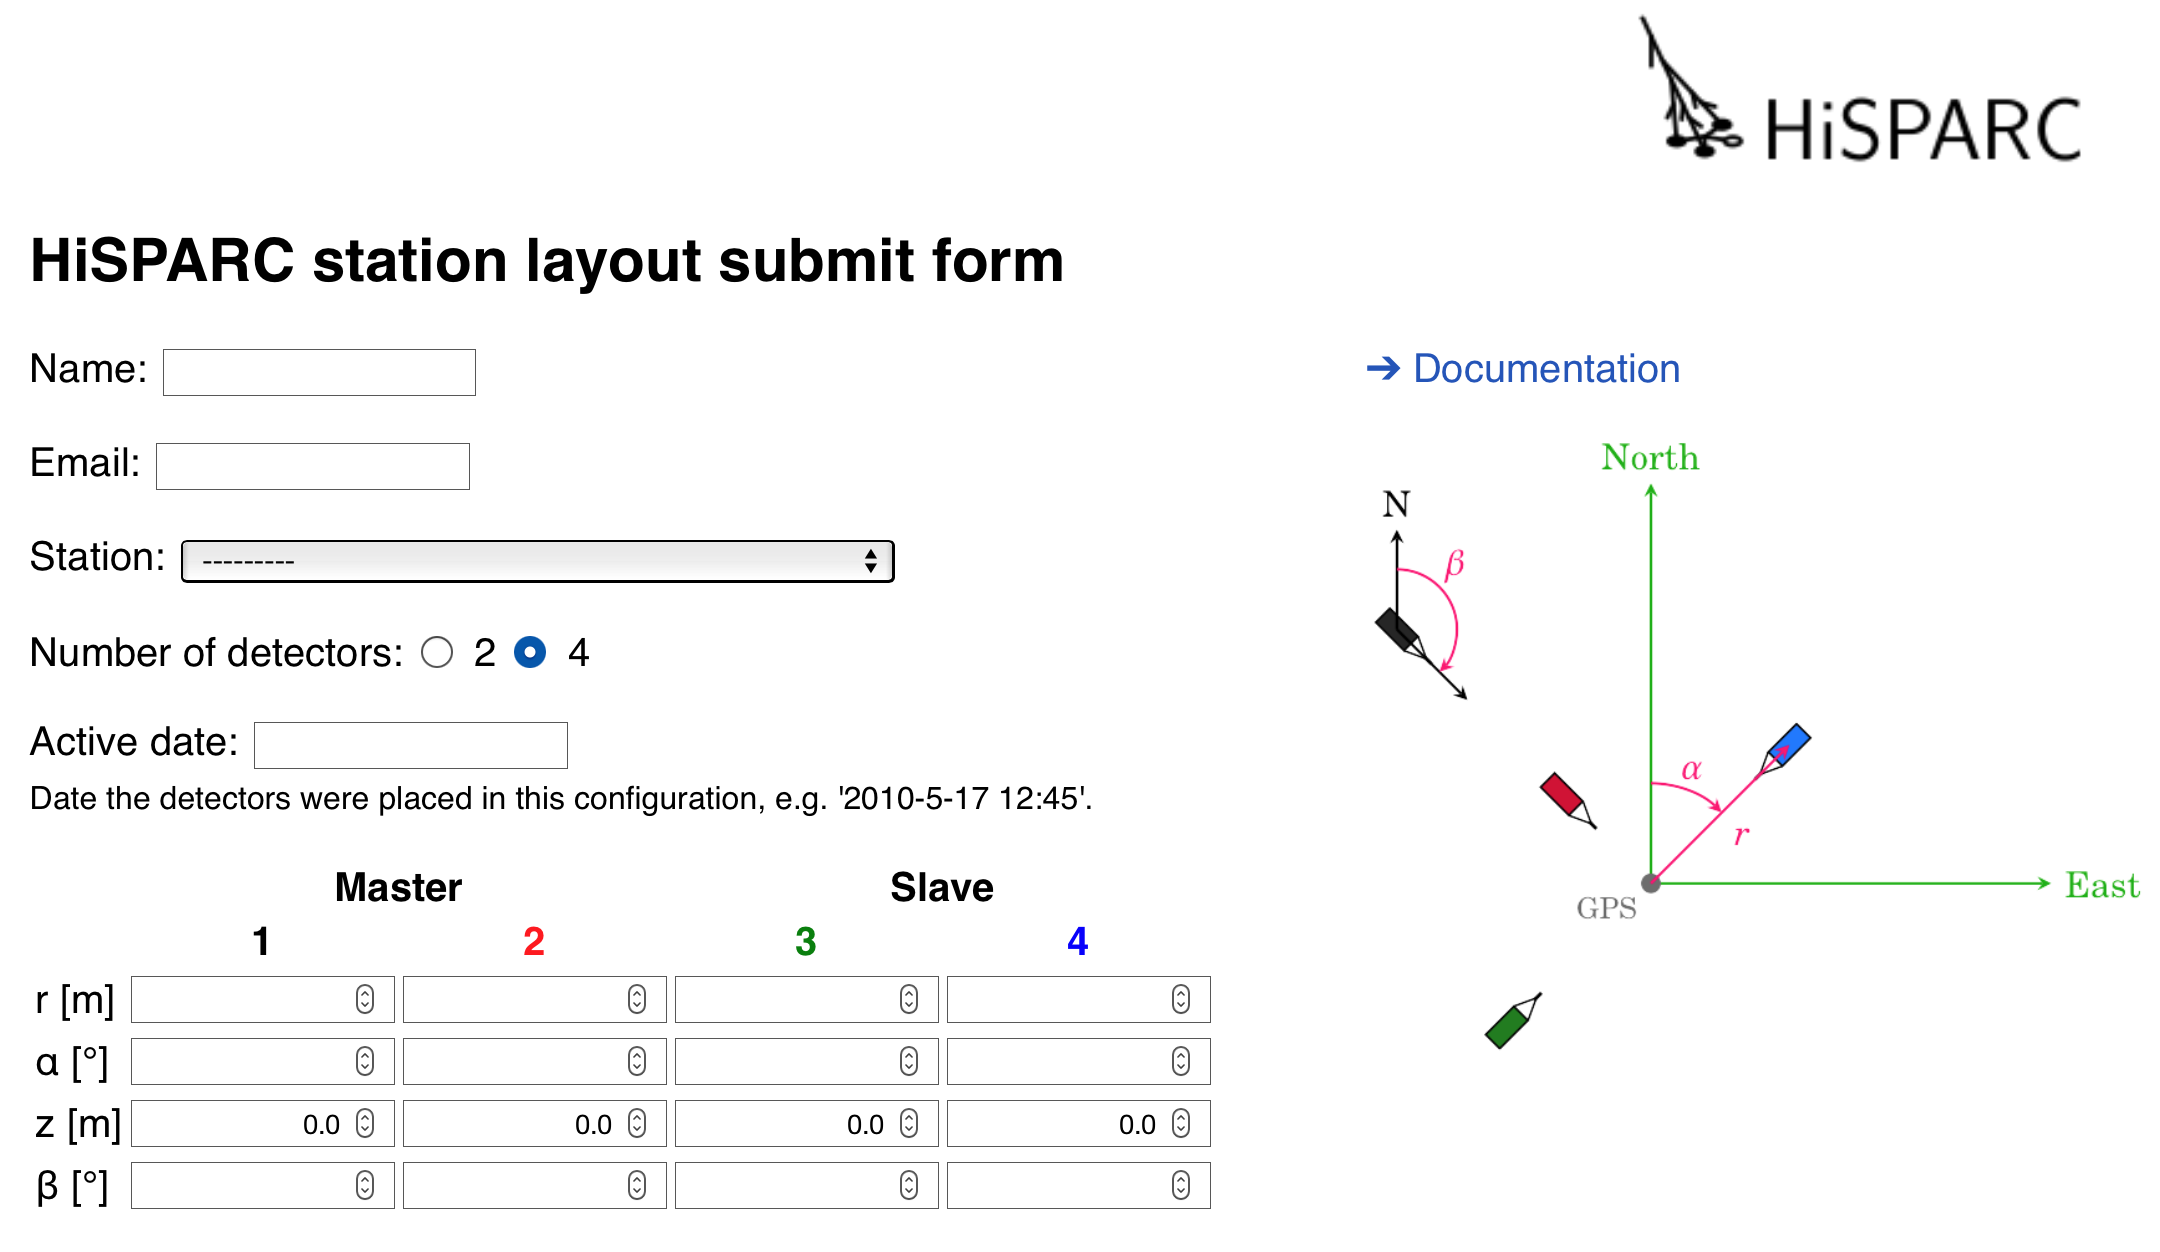
\includegraphics[width=0.9\textwidth]{formulier.png}
    \caption{Het interactieve formulier met een voorbeeld plattegrond.}
\end{figure}

Naast de afstand moeten er nog twee hoeken worden gemeten. Hoek $\alpha$ is de
hoek tussen het noorden en het meetlint van de \gps antenne naar de detector.
Staat de detector ten noorden van de \gps antenne dan meten we een waarde van
\SI{0}{\degree}, staat de detector ten oosten van de \gps antenne dan meten we
\SI{90}{\degree}. Hoek $\beta$ is de hoek tussen het noorden en de lange zijde
van de scintillator in de richting van de Photo Multiplier Tube (PMT) en
lichtgeleider. De kant van de detector met PMT en lichtgeleider is te herkennen
aan de driehoekige vorm van de lichtgeleider en de elektrische aansluitingen
aan de PMT. Wijst kant met de PMT naar het zuiden dan is deze hoek ($\beta$)
\SI{180}{\degree}. Deze metingen kunnen natuurlijk een aantal malen worden
uitgevoerd zodat toevallige fouten kunnen worden verkleind. Indien van
toepassing kan ook het hoogte verschil tussen de \gps en de detectoren worden
gemeten, maar meestal is dat verschil klein en niet significant.

\begin{table}[h]
    \centering
    \begin{tabular}{|>{\centering}p{0.2\textwidth}|>{\centering}p{0.15\textwidth}|>{\centering}p{0.15\textwidth}|>{\centering}p{0.15\textwidth}|>{\centering}p{0.15\textwidth}|}
        \hline
        Detector & 1 & 2 & 3 & 4 \tabularnewline
        \hline
        \hline
        Afstand $r$ [\si{\meter}] &  &  &  & \tabularnewline
        \hline
        Hoek $\alpha$ [\si{\degree}] &  &  &  & \tabularnewline
        \hline
        Hoogte $z$ [\si{\meter}] &  &  &  & \tabularnewline
        \hline
        Hoek $\beta$ [\si{\degree}] &  &  &  & \tabularnewline
        \hline
    \end{tabular}
    \caption{\label{tab:meetgegevens}Meetgegevens}
\end{table}

\paragraph{Opdracht 2:}

Meet de locatie van de detectoren en vul de waarden in Tabel
\ref{tab:meetgegevens} in.

Detector 1 en 2 zijn aangesloten op de \hisparc master unit, te herkennen aan
de \gps aansluiting. Detector 3 en 4 zijn aangesloten op de \hisparc slave
(zonder \gps aansluiting).


\section{Doorgeven van meetgegevens}

De datum en tijd waarop de detectoren zijn geplaatst, of verplaatst,
naar hun huidige positie moeten worden doorgegeven. Ook de gemeten
precieze positie van de detectoren is zeer belangrijk voor de analyse.
Mocht het station ooit verplaatst zijn, dan is het moment van
verplaatsen belangrijk. Voor analyse van een cosmic-ray air-shower
moeten we weten welke positie gebruikt moet worden, dus hoe de
detectoren op dat moment lagen.

De station positie informatie kan worden doorgegeven via een online
formulier: \url{http://data.hisparc.nl/layout/submit/}. Daar moet het
juiste station gekozen worden, de datum (en tijd) waarop detectoren
verplaatst zijn waarna de posities gemeten zijn, en de posities van de
twee of vier detectoren. Zodra je de posities begint in te vullen
verschijnt er onder het formulier een schematische weergave van het
station, controleer of deze weergave overeenkomt met de werkelijke
ligging van de detectoren.

Na het versturen van het formulier wordt eerst het opgegeven mail adres
geverifiëerd. Daarna worden de ingezonden gegevens nagekeken.

\end{document}
